\documentclass[11pt,a4paper]{storm-ai_report}
\addbibresource{references.bib}

\begin{document}

\headerbox{BiMA: Bias-Corrected LightGBM Model for Atmospheric Density Forecasting}
\authordate{Team Bimasakti}{May 24th, 2025}

\begin{participantbox}
  \speaker{Rasyid Ridha}{
    Independent Researcher\\
    Jakarta, Indonesia\\
    rasyidstat@gmail.com\\
  }
\end{participantbox}


\abstractbox{Abstract}{
This report presents BiMA, a Bias-Corrected LightGBM Model for Atmospheric Density Forecasting. BiMA refines the atmospheric density outputs of the recent empirical model, NRLMSIS 2.1, by training an ensemble of LightGBM models on two distinct target representations: ratio and log-ratio between observed and empirical density. This approach combines the generalization capabilities of physically-informed empirical models while mitigating their limitations in capturing complex atmospheric dynamics, particularly during geomagnetic storms. BiMA achieves significant performance improvements compared to the benchmark, with an error reduction of 44\% on unseen test dataset, highlighting its strong generalization and accuracy.
}


\section{Model Report}
\subsection{Model Overview}
\label{subsec:model}

\begin{figure}[h]
\centering
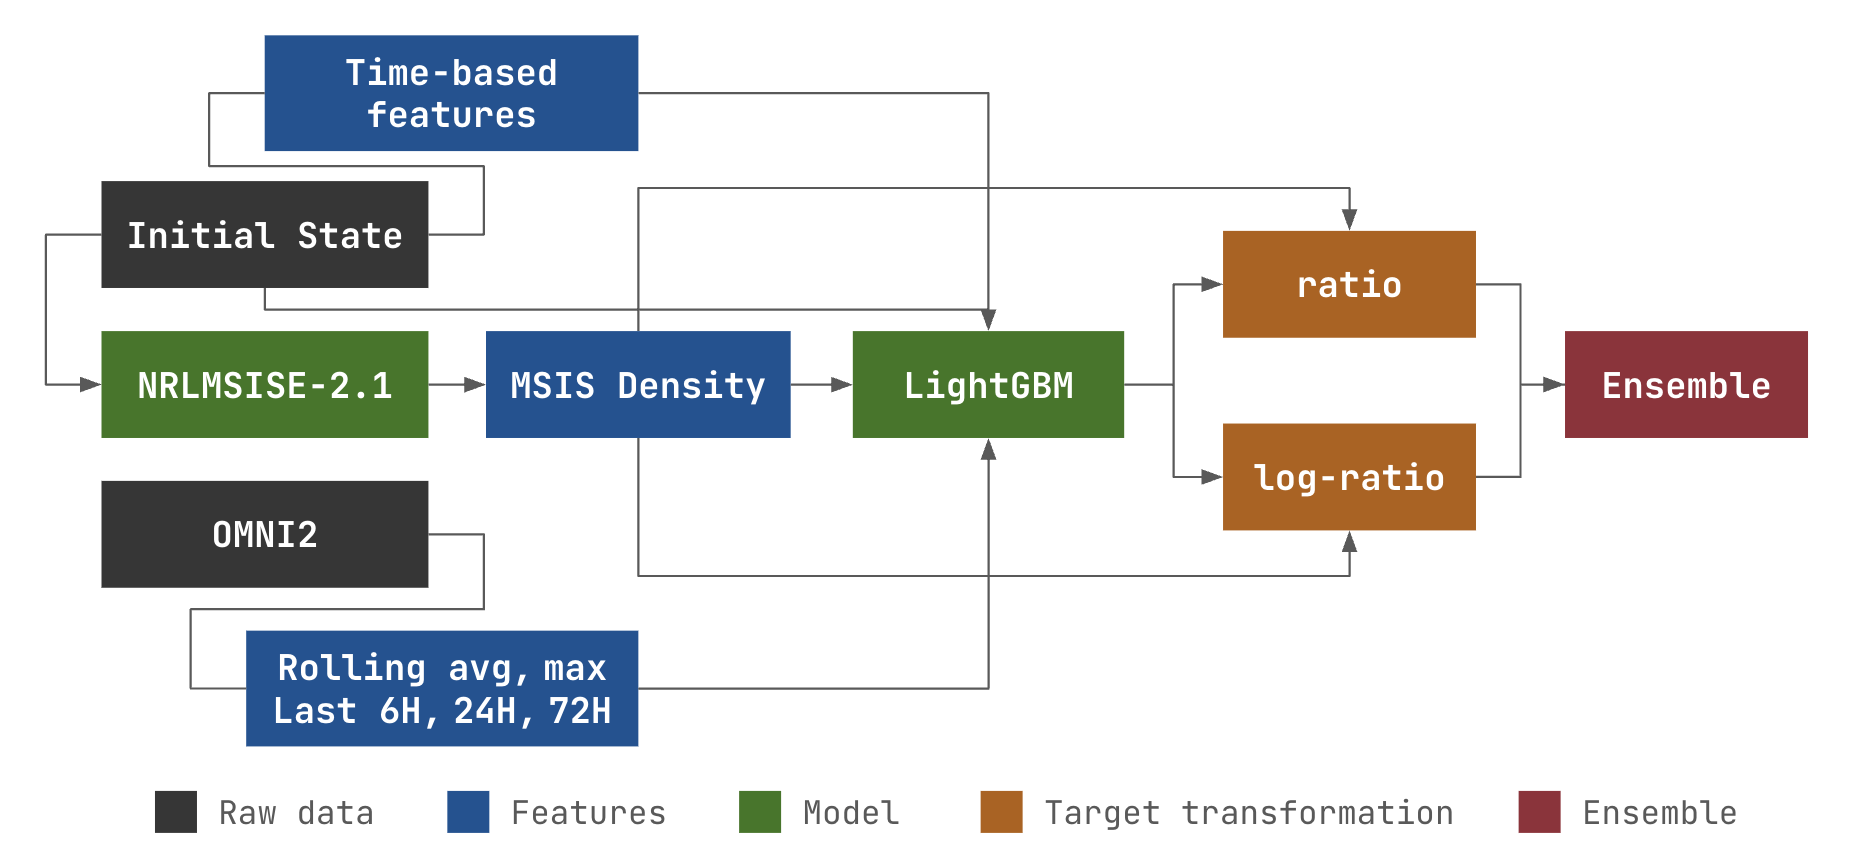
\includegraphics[width=0.7\textwidth]{images/plot/bima-architecture.png}
\captionsetup{width=0.9\textwidth}
\caption{BiMA Architecture Diagram}
\label{fig:architecture}
\end{figure}

BiMA uses a hybrid approach, combining the strengths of both physics-informed models and data-driven methods to achieve robust and accurate atmospheric density forecasts. Physics-informed models are grounded in established physical principles but often struggle to capture complex atmospheric dynamics, particularly during geomagnetic storms. On the other hand, purely data-driven models, while good at learning from training data, may lack generalization in unseen scenarios, especially if the dataset size is limited.

The core principle of BiMA is to learn the systematic bias in the atmospheric density output from the recent empirical model, NRLMSIS 2.1 \cite{Emmert2022NRLMSIS21}, an extension of NRLMSIS 2.0 \cite{Emmert2020NRLMSIS2}. Instead of directly predicting atmospheric density, BiMA refines the outputs of the empirical model by training data-driven models on top of them. This approach, similar to that implemented in \cite{Licata2022MSISUQ}, effectively "calibrates" or "bias-corrects" the MSIS output.

Two models with distinct target representations are used for training: the ratio between observed density and empirical MSIS density ($\rho_{\text{obs}} / \rho_{\text{msis}}$), and the log-transformed version, $\ln(\rho_{\text{obs}} / \rho_{\text{msis}}+1)$, which helps normalize the distribution. LightGBM \cite{Ke2017lightgbm} was selected as the regressor for these models, due to its ability to capture nonlinear relationships, speed, flexiblity, and reproducibility. During inference, predictions from these models are then transformed back, and an average ensemble of both is used to make the result more robust across varied conditions.

A novel aspect of BiMA is its ability to act as a data-driven propagator, refining the initial state density output for each forecast horizon (432 time steps, spanning 3 days at 10-minute intervals). This is necessary as empirical models like MSIS lack a built-in propagator. Instead of using computationally intensive physical orbit propagators, BiMA provides a faster and more resource-efficient solution.

\subsection{Data and Preprocessing}
BiMA was trained using the STORM-AI Phase 1 Public Training Dataset \cite{stormAI}, which includes satellite initial state, OMNI2 space weather data \cite{OMNI2}, and observed atmospheric density from five satellites: CHAMP, GRACE1, GRACE2, GRACE-FO1 and SWARM-A \cite{SWARM}. 

Empirical atmospheric density estimates were computed with \texttt{pymsis} library \cite{Lucas2022pymsis}. Specifically, the estimates are based on the latest empirical model, NRLMSIS 2.1 \cite{Emmert2022NRLMSIS21}, using data inputs from CelesTrak \cite{CelesTrak}, \cite{Matzka2021Kp}, and satellite position at the initial state. These estimates were used both as input and reference values for transforming the target variable (observed density), using two representations mentioned in \nameref{subsec:model}.

A total of 139 input variables were prepared for model training, grouped into the following categories:

\begin{itemize}
    \item \textbf{Satellite Initial State}: This includes raw orbital elements and positional data (latitude, longitude, altitude). Any missing position values were imputed using forward-fill based on known previous state.
    \item \textbf{Time-based Features}: Hour and day-of-year, in both UTC and local solar time, were encoded using sine and cosine transformations to capture cyclical patterns.
    \item \textbf{OMNI2 Space Weather Features}: Rolling aggregations (mean and maximum for last 6, 24, and 72 hours window) of solar activity and geomagnetic indices capture short and medium-term effects. Any missing values remaining after the aggregations were kept as null and handled by LightGBM's internal capability.
    \item \textbf{NRLMSIS 2.1 Atmospheric Density}: The MSIS density estimates at the initial state (computed as described above) were explicitly included as an input feature.
    \item \textbf{Forecast Horizon Encoding}: A numeric indicator of the forecast step (ranging from 1 to 432 for 72 hours at 10-minute intervals) allows the model to act as a propagator which learns forecast horizon specific-biases.
\end{itemize}

\subsection{Training and Validation}

The key to building a strong model lies in choosing an appropriate data split. Initially, a standard k-fold approach was tested to evaluate model performance. However, this setup can lead to overestimated performance, as the model is prone to overfitting from time leakage within the same satellite. As a result, the model may memorize values and time instead of learning meaningful relationships with the input variables. To address this, cross-validation with satellite split was chosen to ensure the model is capable of forecasting density for entirely different satellites, locations, and altitude ranges, ensuring model generalization and reducing overfitting.

In addition, the latest year of data for each satellite-fold was held out as a supplemental evaluation to assess performance on future set, simulating real-world deployment. Both GRACE1 and GRACE2 were included in the same fold due to GRACE1 sample size limitation and the identical nature of both missions. This results into four cross-validated model training runs evaluated on CHAMP, GRACE1/GRACE2, GRACE-FO1, and SWARM-A.

The primary metric to assess model performance is OD-RMSE, aligning with the public leaderboard calculation. However, the baseline reference model used is NRLMSIS 2.1 without propagator. Evaluating the model per satellite and then averaging OD-RMSE ensures the performance metric is scale-invariant. It treats different satellites equally regardless of their absolute density magnitudes, allowing for a better holistic understanding of the forecast performance gain.

For model training, two models, as described in \nameref{subsec:model}, were developed using an identical setup with the objective of minimizing MSE loss. Hyperparameter tuning and feature engineering choices were based on cross-validation performance, emphasizing stability and consistency across satellite performance scores. Finally, an ensemble of models trained on the full dataset was used for inference.

\subsection{Model Performance}

\begin{table}[h]
\centering
\captionsetup{width=0.7\textwidth}
\caption{\centering Model Performance Summary\\CH = CHAMP, G1 = GRACE-1, G2 = GRACE-2, GF1 = GRACE-FO1, SWA = SWARM-A}
\begin{tabular}{|l|ccccc|c|cc|c|}
\hline
\textbf{Model} & \multicolumn{6}{c|}{\textbf{Satellite-Fold CV}} & \multicolumn{3}{c|}{\textbf{Leaderboard}} \\
\cline{2-7} \cline{8-10}
               & \textbf{CH} & \textbf{G1} & \textbf{G2} & \textbf{GF1} & \textbf{SWA} & \textbf{Avg} & \textbf{Public} & \textbf{Private} & \textbf{Phase I} \\
\hline
ratio      & 0.361 & \textbf{0.597} & \textbf{0.497} & 0.111 & 0.332 & 0.380 & 0.743 & 0.408 & 0.693 \\
log-ratio  & \textbf{0.459} & 0.569 & 0.460 & \textbf{0.182} & \textbf{0.408} & \textbf{0.415} & 0.744 & 0.439 & 0.699 \\
ensemble   & 0.420 & {0.593} & {0.490} & 0.152 & 0.379 & 0.407 & \textbf{0.750} & \textbf{0.444} & \textbf{0.704} \\
\hline
\end{tabular}
\label{tab:model_performance}
\end{table}

BiMA consistently outperforms the MSIS benchmark, achieving OD-RMSE of 0.75 on the public test and SSAOD-RMSE of 0.44 on the private test. GRACE-FO1 shows the least improvement, likely because its higher altitude and lower density are more challenging to model, given that the training data is mostly from lower altitudes. Overall, the log-ratio model performs best, particularly for CHAMP, which have highly skewed density values. While the ensemble only adds a small improvement on the leaderboard, it provides more balanced and consistent performance across satellites.

\begin{figure}[h]
\centering
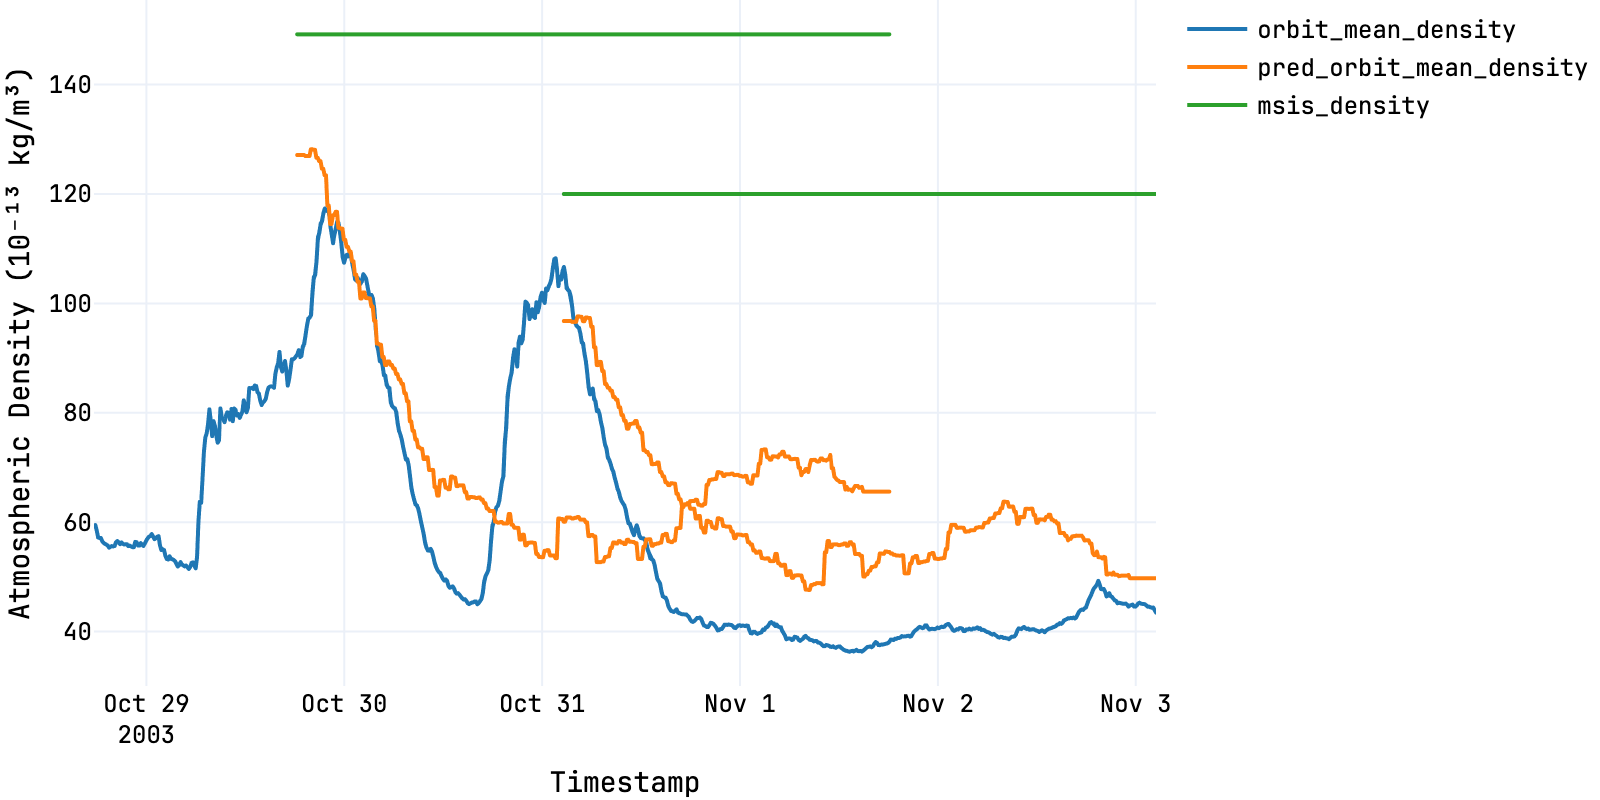
\includegraphics[width=0.8\textwidth]{images/plot/forecast-champ-oct-2003.png}
\captionsetup{width=0.9\textwidth}
\caption{Model Forecasts for CHAMP satellite during 2003 Halloween Solar Storms}
\label{fig:forecast_example}
\end{figure}

Figure \ref{fig:forecast_example} shows the model's capability to forecast atmospheric density under extreme conditions even though CHAMP satellite data was not part of the training data within the cross-validation split. This highlights the model's generalization strength, which is valuable under limited training data points and extreme space weather conditions.

\subsection{Limitations and Future Work}

While BiMA achieves significant performance improvements in atmospheric density forecasting, several limitations and future research areas exist:

\begin{itemize}
    \item Deep learning models, such as LSTMs or Transformers \cite{Briden2023} could potentially improve forecast accuracy, especially at longer horizons. Their inherent ability to capture temporal dependencies and complex patterns in atmospheric dynamics, including responses to geomagnetic storm events, might be better suited than tree-based models.
    \item BiMA currently does not integrate any physics-based propagator, which might lead to physically implausible forecasts, especially at longer forecast horizons. Future work could explore physics-informed machine learning to ensure that the forecast adheres to physical principles.
    \item Including more satellite in-situ data points, especially from varied altitudes, or using synthetic data, could further improve generalization.
    \item Incorporating uncertainty estimation \cite{Licata2022MSISUQ} and forecast explainability would provide valuable guidance for operational use.
\end{itemize}


\subsection{Conclusion}

This work highlights BiMA as a fast, robust and accurate model for forecasting atmospheric density, combining the strengths of physics-informed models with machine learning correction. The model performs well across a wide range of conditions, including during extreme space weather, and generalizes effectively to satellites and altitudes not seen during training. BiMA also generates forecasts more quickly as it does not rely on physical orbit propagators, making it suitable for real-time forecasting applications. These qualities support its use in operational settings where timely updates are essential, helping reduce risks such as satellite drag and orbital collisions.

\subsection{Code Availability}

All code used to generate the results in this report, including data preprocessing, feature engineering, model training, and evaluation, will be released upon competition on \faicon{github} \href{https://github.com/rasyidstat/BiMA}{BiMA GitHub repository}.


\printbibliography

\end{document}
